\documentclass[12pt,twoside,notitlepage]{report}
\usepackage{a4}
\usepackage{verbatim}
\usepackage{graphicx}
\usepackage[font={small,it}]{caption}
\usepackage{subcaption}
\usepackage{pdfpages}
\usepackage{amsmath}
\usepackage{bm}
\raggedbottom                           % try to avoid widows and orphans
\sloppy
\clubpenalty1000%
\widowpenalty1000%

\addtolength{\oddsidemargin}{6mm}       % adjust margins
\addtolength{\evensidemargin}{-8mm}

\renewcommand{\baselinestretch}{1.1}    % adjust line spacing to make

\begin{document}

\bibliographystyle{plain}


%%%%%%%%%%%%%%%%%%%%%%%%%%%%%%%%%%%%%%%%%%%%%%%%%%%%%%%%%%%%%%%%%%%%%%%%
% Title


\pagestyle{empty}

\hfill{\LARGE \bf Karina Palyutina}

\vspace*{60mm}
\begin{center}
\Huge
{\bf Machine learning inference of search engine heuristics} \\
\vspace*{5mm}
Part II Project \\
\vspace*{5mm}
St Catharine's College \\
\vspace*{5mm}
\today  % today's date
\end{center}

\cleardoublepage

%%%%%%%%%%%%%%%%%%%%%%%%%%%%%%%%%%%%%%%%%%%%%%%%%%%%%%%%%%%%%%%%%%%%%%%%%%%%%%
% Proforma, table of contents and list of figures

\setcounter{page}{1}
\pagenumbering{roman}
\pagestyle{plain}

\chapter*{Proforma}

{\large
\begin{tabular}{ll}
Name:               & \bf Karina Palyutina                       \\
College:            & \bf St Catharine's College                     \\
Project Title:      & \bf Machine learning inference of search engine heuristics \\
Examination:        & \bf Part II Project        \\
Word Count:         & \bf \footnotemark[1]     \\
Project Originator: & Dr Jon Crowcroft                    \\
Supervisor:         & Dr Jon Crowcroft                  \\ 
\end{tabular}
}
\footnotetext[1]{This word count was computed
by {\tt detex diss.tex | tr -cd '0-9A-Za-z $\tt\backslash$n' | wc -w}
}
\stepcounter{footnote}

\newpage


\section*{Original Aims of the Project}


\section*{Work Completed}


\section*{Special Difficulties}

\section*{Declaration of Originality}

I, Karina Palyutina of St Catharine's College, being a candidate for Part II of the Computer
Science Tripos , hereby declare
that this dissertation and the work described in it are my own work,
unaided except as may be specified below, and that the dissertation
does not contain material that has already been used to any substantial
extent for a comparable purpose.

\bigskip
\leftline{Signed }

\medskip
\leftline{Date }

\cleardoublepage

\tableofcontents


%%%%%%%%%%%%%%%%%%%%%%%%%%%%%%%%%%%%%%%%%%%%%%%%%%%%%%%%%%%%%%%%%%%%%%%
% now for the chapters

\cleardoublepage        % just to make sure before the page numbering
                        % is changed

\setcounter{page}{1}
\pagenumbering{arabic}
\pagestyle{headings}

\chapter*{Introduction}
\addcontentsline{toc}{chapter}{Introduction}
This project is inspired by increasing importance of search engine rankings.
Today major search engines given a query return web pages in an order
determined by secret algorithms. Such algorithms are believed 
to incorporate multiple unknown factors.
For instance, Google claims to have over 200 unique factors that influence a
position of a webpage in the search results relative to a query
\footnote{http://www.google.com/competition/howgooglesearchworks.html}. Only
a handful of these factors are disclosed to the webmasters  in the form of very
general guidelines. Moreover, the Google algorithm in particular is updated
frequently. However, most of the knowledge around the area amounts to
speculation. Despite the fact that it is possible to pass a vast number of
queries through the black box of any existing search engine,the immensity of
the search space, and instability of such algorithms make them impossible to
reverse engineer.

Machine learning is a natural approach to inferring the true algorithm from a
subset of all possible observations. However, applying machine learning
techniques to real search engines would be hardly effective, as the dynamic
nature of the algorithms and the web as well as lack of meaningful feedback
would prevent incremental improvement: when there are as many as 200 features
in question, false assumptions made by a learner may have an unpredictable
effect on its performance.

More generally, there are certain ambiguities associated with machine learning,
which are 'problem-specific'. For example, it proves difficult to decide how
much training data is necessary, as well as and selecting it to avoid
over/under-fitting\cite{domingos}. Similarly, it is not straightforward which
machine learning technique is best for a particular problem.

This project is concerned with application of machine learning techniques to
search engines. The aim of the project, in particular,  is to explore how
machine learning techniques can be used effectively to infer algorithms from
search engines. To address the limitations imposed by existing search engines,
part of the task is to develop a toy search engine that allows me to comtrol
the nature and complexity of used heuristics. Such transparency addresses the
problems stated above and, more importantly,  allows for useful evaluation of
machine learning techniques by providing meaningful feedback.

Even though this study does not attempt to reverse engineer any existing
heuristics, the results can be applied to such an ambitious task.
Moreover, such a framework is potentially more general and can be used for a
range of problems.

\newcommand\todo[1]{\textcolor{red}{\textbf{TODO: #1}}}
\todo{overview of the chapters here.}

\cleardoublepage
\chapter{Preparation}
This chapter describes work that has been done before coding was started.  In
particular, it focuses on the reasoning behind the design of the system to be
implemented. The first section is devoted to research undertaken to determine
what can be done and how best to do it. The second section formulates the
system requirements, namely formalizes everything that is developed in this
project. The last section outlines the particulars of the software engineering
approach to be adopted by this project.

\section{Formulating the Goals}
\label{prep}
A particular difficulty in this project has been in planning what has to be
done. Due to the exploratory nature of the project the course of action had to
be predominantly determined by the outcome of a current tactic. Moreover, the
unknowns originating from the machine learning further complicated matters. 

\subsection{System Overview}

To achieve the goal of the project, a machine learning techniques comparison
framework was necessary. In the Introduction I mentioned the benefit of having
a transparent system as an object of learning. To further justify this
decision, it is worth mentioning that  generalisation using machine learning is
different from most optimization problems in that the function that is being
optimized is out of our reach, and all that is visible to the machine learner
is the training error. Because our goal is not the correct classification of
real data, but identifying the means to correct classification, it is important
that informed choices are made towards improvement of the learner. Taking this
into account, knowing the function that we want to learn and having direct
control over it  will guide the improvement of the search engine. 

This argument motivates a system in three parts: a search engine, a machine
learner and a parser to mediate between the two.  Figure \ref{overview}
illustrates the proposed learning system. Training data is a set of web pages
set aside specifically for training purposes.  

\begin{figure}
\centering
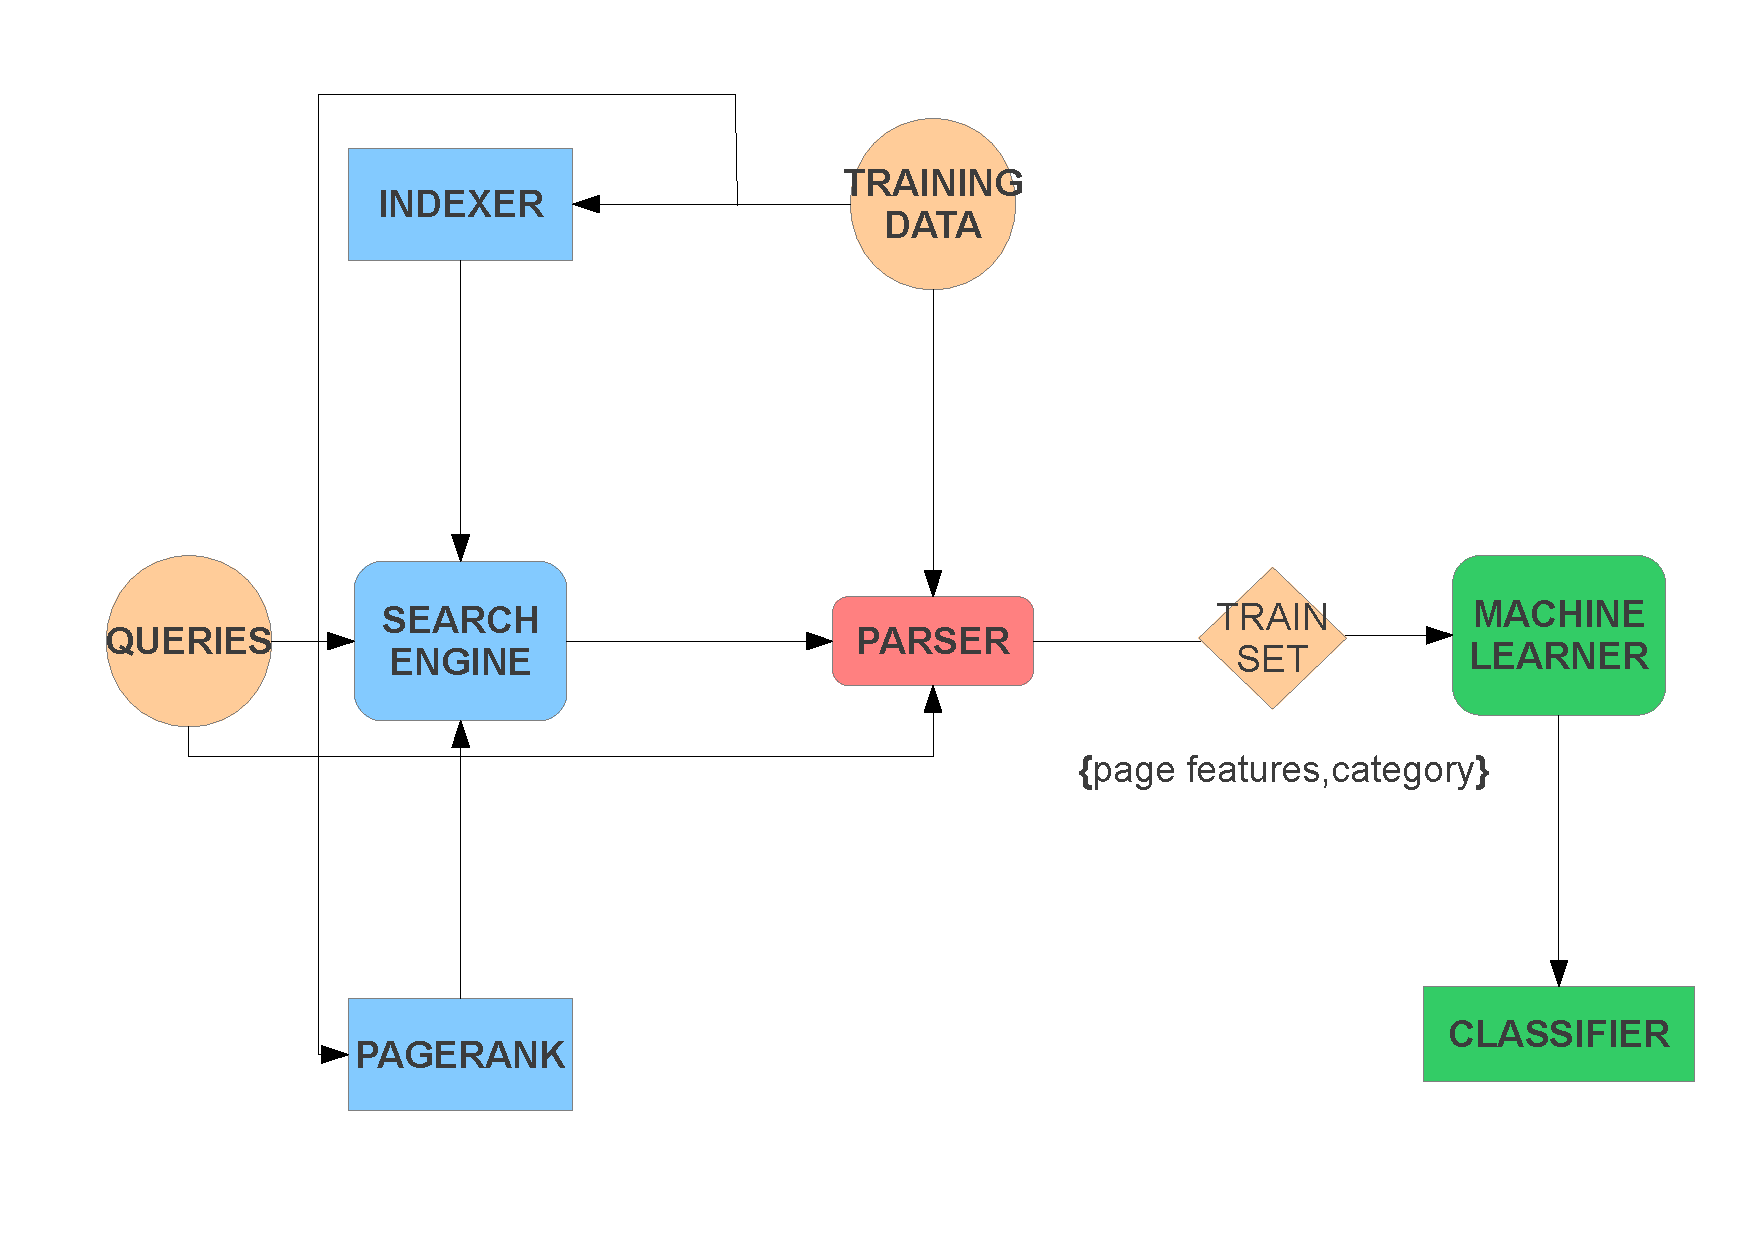
\includegraphics[scale=0.5]{figs/overview.pdf}
\caption{Overview of the system. Three major parts from left to right are search engine,
parser and machine learner.}
\label{overview}
\end{figure}

\subsubsection*{Choice of Programming Language}

When choosing a programming language, main considerations reduced to library
availability and simplicity. The project imposes no special  requirements on the
language, apart from, perhaps, library infrastructure for parsing web pages.
Python is simple language with extensive library support. As
for efficiency, all the mathematical operations in this project rely on python
math libraries, which are implemented in C. I have not programmed in Python
before the project, so a slight overhead was caused by having to learn a new
language.

\subsubsection*{Data}
Web pages used as Training and Test data are not required to have any special
properties, but diversity and typicality are seen as advantageous. As for the
size of the training data, Domingos \cite{domingos} suggests that a primitive
learner given more data performs better than a more complex one with less data.
This, of course, is under certain assumptions of data quality, namely the
assumption that the training data is a representative subset of all the
possible data. Intuitively, provided there is no bias in data gathering, more
data implies better generality. I have started with a training set spanning an
order of a few thousands of pages, however, in practice, I found that there is
no particular improvement beyond a thousand pages. \todo{Link to relevant part
or example data here?}

\subsection{Search Engine}

Next important decision regarded the search engine.  Originally, I considered
using open source existing engines, in particular, Lucene. Even though I could
freely modify it for the purposes of the project, the complexity of it was
superfluous. I saw writing a simple search engine as a more beneficial
exercise, as developing it in the first place potentially gives an insight into
the problem.

Functionally our search engine is a black box that takes a set of webpages and
a set of queries and outputs an order. The order is determined by the features
of the page, which together make up a score. The score is the
function we want to infer using the ranking assigned by the search engine,
however, we are only given the order as evidence. Machine learning paragraph
below will address this issue in more details.

In general there are two aspects of information retrieval that have to be
accounted for: precision and recall. Precision is the fraction of retrieved pages that
are relevant to the query, whereas recall is the fraction of relevant
documents that are retrieved. Even though both are important for a good search
engine, but in practice, the web is very large, and so precision, or even
precision at n\footnote{Precision at n only evaluates precision with respect to
n topmost returned pages.}) has become
more prominent in defining a good search engine: very rarely the user actually
browses returns that are not in the top few tens of returned pages. Therefore, 
modern search engines tend to focus on high precision at the expense of recall
\cite{GOOGLE}. Therefore, we will concentrate primarily on precision, when
designing a search engine.

\todo{Why pagerank?}
The PageRank algorithm was implemented as described in the original paper
by Page and Brin\cite{pagerank}.


\subsection{Machine Learning}

I have now covered main peripheral decisions, but it is machine learning that
constitutes the central part of the project. The field was completely new to me
to start with, so research of different techniques was a big part of the
preparation.

It is generally recommended that the simplest learners are tried
first\cite{domingos}. Of all learners Naive Bayesian is one of the most
comprehensible.This in itself is a major advantage according to the Occam's
razor principle, which finds ample application in machine learning.

\subsubsection*{Naive Bayes}

Naive Bayes is a probabilistic classifier based on the Bayes Theorem. The
posterior probability \(P(C|\vec{F})\) denotes the probability that a sample
page with a feature vector \(\vec{F}=(F_1,F_2,\dots,F_n)\) belongs to class C.
The posterior probability is computed from the observable in the training data: the prior
probability \(P(C)\) -- the unconditional probability of a page belonging to
the class C, the likelihood \(P(\vec{F}|C)\) and the evidence \(P(\vec{F})\):
\begin{equation}
P(C|\vec{F}) = \frac{P(C)P(\vec{F}|C)}{P(\vec{F})}
\end{equation}

The simplicity of Bayesian approach owes to the conditional independence
assumption: each \(F_i\) in \(\vec{F}\) is assumed to be independent of one
another to get \(P(\vec{F}|C)=P(F_1|C)*P(F_2|C)*\dots*P(F_n|C)\). This leads to a concise classifier definition:
\begin{equation}
\hat{C}= argmax_C P(C)\prod_{i=1}^{n}P(F_i|C)
\end{equation}
where \(C\) is the result of classification of a page with feature vector
\(F_1,F_2,\dots,F_n\).

In practice, the crude assumption rarely  holds and is likely to
be violated by our data, as we expect features of pages to be interdependent.
However, it has been shown that Naive Bayes performs well under zero-one loss
function in presence of dependencies\cite{OPTIM}. This has a few
implications for this project, particularly, on evaluation methods 

As we have seen, Naive Bayes assigns probabilities to possible classifications
in the process of classifying. Even though it generally performs well in
classification tasks, these probability estimates are poor \cite{domingos96}.
However, despite poor probability estimates, there exist several frameworks,
which make use of Bayesian classification and achieve decent performance in
ranking. For example, Zhang \cite{zhang04} experimentally found that Naive
Bayes is locally optimal in ranking. The paper defines a classifier as locally
optimal in ranking a positive example E if there is no negative example ranked
after E and vice versa for a negative exaple. A classifier is global in ranking
if it is locally optimal for all examples in the example set: in other words,
it is optimal in pairwise ranking.  It is particularly interesting that the
paper discovered that Naive Bayes is globally optimal in ranking on linear
functions that have been shown as not learnable by Naive Bayes\footnote{m-of-n
concepts and conjunctive concepts can't be learnt by Naive Bayes classifier but
can be optimally ranked by it according to Zhang \cite{zhang04}.}.
Another framework for ranking \cite{bayesrank} is based on Placket-Luce model, which reconciles
the concepts of score and rank. This framework is based on minimizing the Bayes
risk over possible permutations.

Existence of such frameworks suggest that Naive Bayes is an adequate choice
for this project. Classification is frequently opposed to regression, so
another approach covered by this project is Support Vector Regression. In
particular, \(\epsilon\)-Support Vector Regression.

\subsubsection*{\(\epsilon\)-Support Vector Regression}
\todo{Justify why SVM: shortcomings of NB, many dimensions, kernel functions}
While the binary classification problem has as its goal the maximization of the
margin between the classes, regression is concerned with fitting a hyperplane
through the given training sequence.  A training sequence is a set of training
points \(D = \{ (\mathbf{x_1},t_1), (\mathbf{x_2},t_2), ... ,
(\mathbf{x_l},t_l) \}\) where \( \mathbf{x_i} \in R^n \) is a feature vector
holding features of pages and \( \mathbf{t_i} \in R \) is the corresponding
ranking of each page.

\begin{figure}
  \centering 
  \includegraphics[width=120mm]{epsilon.jpg}
  \caption{TODO: plot these yourself!} 
  \label{eps} 
\end{figure}

In simple linear regression the aim is to minimize a regularized error
function. We will be using an \(\epsilon\)-insensitive error function(see
Figure \ref{eps} (a)).

\(E_\phi(y(\mathbf(x)-t)) = \left\{ \begin{array}{l l} 0 & \quad \text{if
\(|y(\mathbf{x})-t)|<\epsilon\)}\\ |y(\mathbf{x})-t)|-\epsilon & \quad
\text{otherwise} \end{array} \right.\)

where \(y(\mathbf(x) = \mathbf{w^T}\phi(\mathbf{x})+b\) is the hyperplane
equation (and so \(y(\mathbf{x}) \) is the predicted output) and \(t_n\) is the
target (true) output.

The regression tube then contains all the points for which \(
y(\mathbf{x_n})-\epsilon \leq t_n \leq y(\mathbf{x_n})+\epsilon \) as shown in
Figure \ref{eps}(b).

To allow variables to lie outside of the tube, slack variables \(\xi_n \geq
0\)and \(\xi_n^* \geq 0\) are introduced.  The standard formulation of the
error function for support vector regression (ref Vapnik 1998) can be written
as follows:

\begin{gather} E= C\sum_{n=1}^{N}(\xi_n+\xi_n^*)+\frac{1}{2}\|\mathbf{w}\|^2
\end{gather}

\(E\) must be minimized subject to four constraints:

\begin{gather} \xi_n\geq 0,\\ \xi_n^*\geq 0,\\ t_n \leq
  y(\mathbf{x_n})+\epsilon+\xi_n,\\ t_n \geq y(\mathbf{x_n})-\epsilon-\xi_n^*,
\end{gather}

This constraint problem can be transformed into its dual form  by introducing
Lagrange multipliers \(a_n \geq 0, a_n^* \geq 0\).  The dual problem involves
maximizing

\begin{gather} \label{eq:maxim}  L(\mathbf{a},\mathbf{a^*}) =
  -\frac{1}{2}\sum_{n=1}^{N}\sum_{m=1}^{N}(a_n-a_n^*)(a_m-a_m^*)K(\mathbf{x_n},\mathbf{x_m})
\end{gather} \begin{gather*} -\epsilon\sum_{n=1}^{N}(a_n+a_n^*) +
  \sum_{n=1}^{N}t_n(a_n-a_n^*) \end{gather*}

where \(K(x_n,x_m) \) is the kernel function, \(t_n\) is the target output,

subject to constraints

\begin{gather}
  \sum_{n=1}^{N}(a_n-a_n^*)=0,\\
  0\leq a_n,\; a_n^*\leq C,\;\;    n=1,...,l 
\end{gather}


\subsubsection*{Evaluation methodology}
Two proposed techniques Naive Bayes and SVM regression are quite different, so
comparing them is potentially erroneous. However, comparisons can be done
within each method, as there is a lot of scope for variety of implementations
in each.
As a baseline for the Bayesian approach, a very primitive ranking model will be
used. We will simply disregard the scoring function behind the rank and
directly infer the ranking function instead. More sophisticated ranking models
can then be compared to this basic performance.
Figure \ref{eval} shows an evaluation framework for Naive Bayes.  The Test Data
is the data carefully set aside at the beginning that is never exposed to the
learner. 

\begin{figure}[h]
\centering
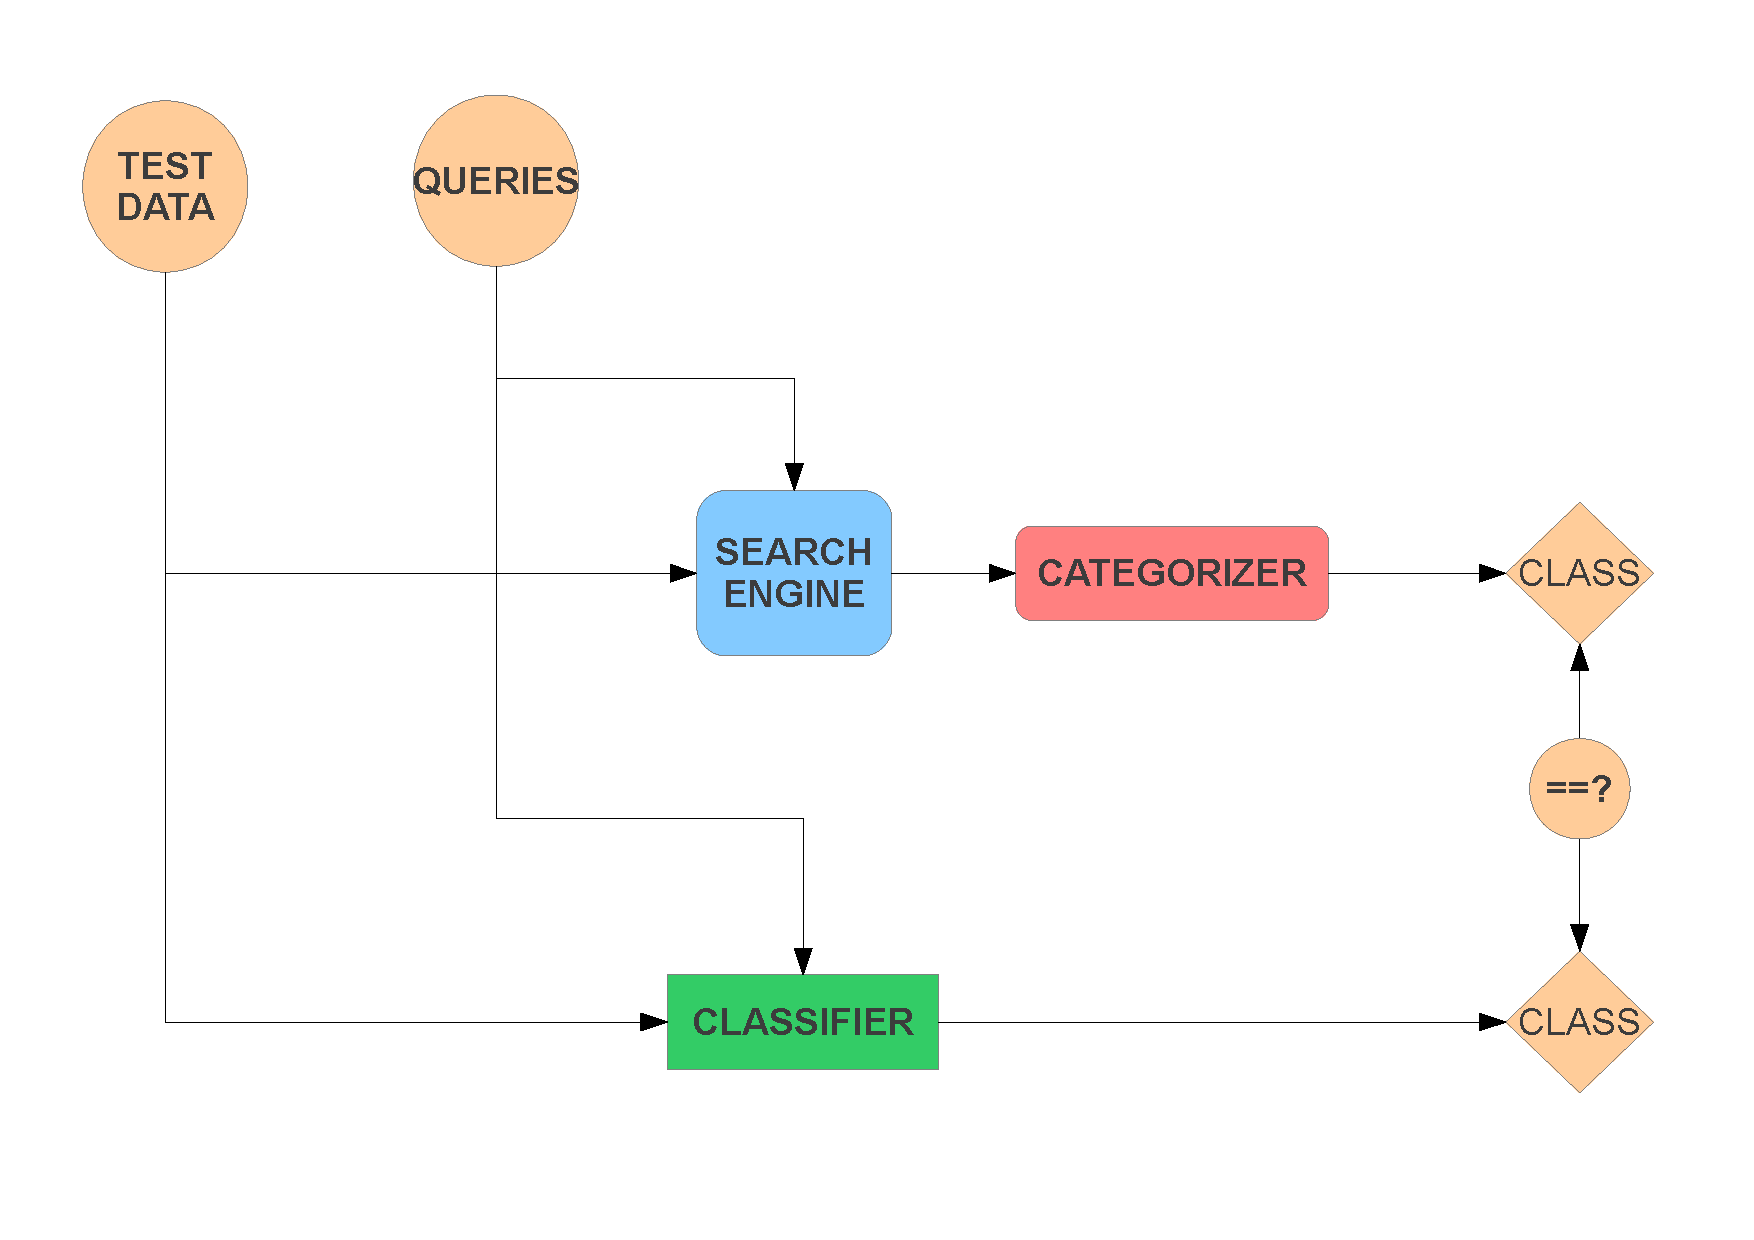
\includegraphics[scale=0.5]{figs/eval.pdf}
\caption{Evaluation system. }
\label{eval}
\end{figure}
For an SVM learner the baseline can be set to the performance using a linear
kernel below.

\begin{gather*}
K(x,y) = x \cdot y
\end{gather*}
where `\(\cdot\)' denotes the dot product.

This is expected to be very high for linear heuristics but a lot lower for
non-linear ones.

\section{Development Strategy}
While the set up of Part II projects encourages waterfall-like development
model, this project takes an iterative approach. The first iteration renders a
prototype: a primitive search engine with a Naive Bayesian baseline classifier.
The next iteration modifies each part of the system towards a more complex
solution. Evaluation is performed at each iteration. Within each  iteration the
development follows the evolved waterfall model -- the incremental build model.
Each increment represents a functionally separate unit of the system: a search
engine, a learner, a parser and an assessment module. Increments are developed
sequentially and regression testing is performed separately before integration.

The backup of the code is twofold: every time a substantial change is made a remote
version control repository is updated to hold the newest version. Regularly both the code and
the data used and obtained during evaluation are also backed up onto an
external hard drive. 

During the development of the learners a development pool of pages will
be used, which must be disjoint with the Training or Test data. This ensures
that no optimization is tailored to the data used for evaluation. 

\subsection*{Requirements Analysis}
The resulting system must comply with the requirements stated below. 
\begin{itemize}
  \item{A search engine, which given a query must return a relevant subset of
      pages within 10 seconds in an order corresponding to a given heuristic, which can also be
  supplied to the search engine.}
  \item{Search engine must base ranking decisions on both dynamic
      (query dependent) and static (query independent)
    page features.}
  \item{A machine learner must be sufficiently isolated from the search engine
    through an encapsulating interface to avoid the possibility of undesirable interaction.}
  \item{Machine learners must be able to process thousands of pages in a
    reasonable time.}
  \item{The evaluation module must write results to persistent storage.}
\end{itemize}
\cleardoublepage
\chapter{Implementation}
This section describes parts of the system that I have implemented.
\todo{overview}

\section{Data}
Development, Test and Training data for this project was implemented
Separate directories..

\section{Search Engine}

The first basic block of the system -- the search engine -- can be logically
split into two main parts: an indexer and a sorter. Because we concentrate on
precision, as discussed in the Preparation chapter, we will assume for
simplicity that all relevant documents are returned. This allowed me to an use
existing library implementation of the indexer and focus on the sorter.

\subsection*{Indexer}

The requirements on the indexer included flexibility, speed of indexing and
retrieval, simplicity and usability.  The `Whoosh' python library provides all
of these, so I used it to build an indexer. `Whoosh' is an open source indexing
library, so I had the option of modifying any part of it. It is  built in pure
Python, so it has a clean pythonic API. Its primary advantage is fast indexing
and retrieval, although we are mostly concerned with retrieval speed, as
indexing is done rarely. The predecessors of `Whoosh' have served as the basis
of well-known browsers such as Lucene, so it is also a powerful indexing tool,
should I have needed more sophistication.

I have defined a very simple schema for indexing. Perhaps, one notable detail
is that `Whoosh' can store timestamps with the index, which enabled me to
provide both clean and incremental index methods. The incremental indexing
relies on the timestamp stored with the index and compares it to the
last-modified time provided by the file system. The user can specify whether
indexing has to be done from scratch or updated to accommodate some document
changes or document addition/deletion. I haven't originally expected to need an
incremental indexing capability, but throughout the project it has permitted
for a significant speedup.

Previously, I have defined the sorter as a logical unit that provides ranking to the
retrieved documents. For the first prototype, the sorter returned the pages in
the order of decreasing pagerank.
Subsequently, the sorting has been decoupled from retrieval and is described in
more detail in the Parser section.

\subsubsection*{PageRank} 
The PageRank vector is computed using matrix inversion. All matrix operations
were performed with the help of the python numerical library `numpy'.  Take t
to be the teleportation probability, s=1-t is the probability of following a
random link, E is the teleportation probability: equiprobable transitions, as
using non-personalized pagerank (see Preparation), \(E_i,j = 1/N\) for all i,
j. G is a stochastic matrix holding the link structure of the data, such that 
\begin{equation*}
  G_i,j = \begin{cases}
    1/L & \text{there is a link from i to j and L = number of links from i}\\
    0   & \text{there is no link from i to j}
  \end{cases}
\end{equation*}
Then M is a stochastic matrix representing the web surfer activity, such
that \(M_i,j\) is the probability of going from page i to page j, 
\begin{equation} \label{1}
  M = s*G +t*E
\end{equation}
In one step the new location of the surfer is described by the distribution Mp.
We want to find a stationary distribution p, so must have
\begin{equation}\label{2}
  p = M*p
\end{equation}
Substituting \ref{1} into \ref{2}
\begin{equation} \label{a}
  p = (s*G+t*E)*p = s*G*p + t*E*p
\end{equation}
Rearranging equation \ref{a} gives
\begin{equation}
  p*(I-s*G) = t*E*p
\end{equation}
where I is the identity matrix

We can express E*p as P where P is a vector
\([\overbrace{1/N,1/N,\dots,1/N}^N].T\),as members of p must sum to one.
So computing pagerank amounts to
\begin{equation}
p  = t*(I-s*G)^{-1}*P
\end{equation}
where \((I-s*G)^{-1}\) denotes a matrix inverse operation.

This solution is simple at the expense of being slow. Although computing
inverse of a matrix is computationally expensive, we don't need to scale beyond
a few thousands of pages.  To avoid recomputation, I used python object
serialization module - Pickle to store the pagerank vector for each directory.
The resultant performance was actually very reasonable, the time spent
computing pagerank was insignificantly small in comparison to the time spent
crawling the directory.

\todo{Load class method}
\todo{byname array}
\subsubsection*{Crawler}
The matrix G, used for the pagerank computation, represents random link
following activity. To obtain such a link structure each page has to be parsed,
and all links recorded. Because our data is obtained from a single source page
by a Wget spider, every page in a directory is guaranteed to be discovered by a
spider.

The Crawler class recursively traverses the pages depth first starting with the seed page,
the same as the seed page used for recursively downloading the pages from the
web. To make sure each page is only explored once, a dictionary is used to
hold pairs of absolute path, which uniquely identifies the page, and a
numerical value corresponding to the timestamp when the page has been first
discovered.
\todo{link conversion and parsing}
Although every page has a unique path, the links to other pages are relative.
Such links need to be normalized to maintain consistency.
A page object is used to encapsulate path complexity: all link paths are
converted to absolute paths before addition to the dictionary.
All outbound links are stored with the page in a Set datastructure,
such that no link is added more than once. 

To produce the stochastic matrix G, we start with an empty NxN matrix, where N
is the total number of pages. We assume that whenever a surfer encounters a dangling page -- a page that has no
outbound links -- a teleportation step occurs. Therefore, every dangling page
links to every page in the pool including itself with equal probability 1/N. For non-dangling
pages, all links are assumed equiprobable and all pages that are not linked to
have probability of 0. So if page A links to pages B and C, but not itself or
D, its row in G is described by the Table \ref{tab}.

\begin{table}
    \begin{center}
      \begin{tabular}{|l|r|}
        \hline
        Page & A \\ \hline
         A &  0  \\ \hline
         B & 1/2 \\ \hline
         C & 1/2 \\ \hline
         D & 0   \\ \hline
      \end{tabular}
      \caption{Illustration of non-dangling pages: B and C share A's `importance' equally.\label{tab}}
  \end{center}
\end{table}

\section{Machine Learning}
In the course of this project two distinct machine learning algorithms have
been used. The design goals for the implementations were as usual: speed and
correctness. Another important aspect of the design is that the system and the
machine learning modules must be sufficiently decoupled. This is an issue of
scalability and code reuse. The implication on the machine learner
implementations is that both must communicate with the system via the same
interface.
The rest of the section describes in detail how the machine learners have been
implemented.

\subsection{Naive Bayes}
In Section \ref{prep} it has been shown that Naive Bayesian is a good learner
to implement for the first prototype, so a very quick implementation was
preferable to make sure the system can potentially function as intended. Due to
its simplicity and popularity, Naive Bayesian is widely available in the
libraries. Because the implementation of this module is straightforward, not
central to the project, I decided to use one of many existing python
implementations. 

The \textit{nltk} library implementation was particularly appealing as it offers a very
concise interface. A classifier object is initialised by the \texttt{train}
method on the \texttt{NaiveBayesClassifier} class. The format of the training
set is defined as a list of tuples of featuresets and labels, e.g.
\\ \textit{[(\(featureset_1, label_1\)),\( \cdots\), (\(featureset_N,
label_N\))]}. 
The \texttt{train} method simply computes the prior -- the probability distribution over
labels P(label) and the likelihood -- the conditional probability
P(\(featureset=f|label\)) by simply counting and recording the relevant instances. The method
outputs a \texttt{NaiveBayesClassifier} instance parametrized by the two
probability distributions.

P(features) is not computed explicitly, instead, a normalizing denominator
\ref{normal} is used.

\begin{equation}
  \sum_{l \in labels}(P(l)P(featureset_1|l)\cdots P(featureset_N|l))
\end{equation}

The \texttt{classify} method on the \texttt{NaiveBayesClassifier} object takes
exactly one featureset and returns a label which maximizes the posterior
probability P(label|featureset) over all labels.
Previously unseen features are ignored by the classifier, so that to avoid
assigning zero probability to everything.

The only tangible difficulty with the implementation was the framework in which
classification is done. The Parser was `written around' the interface of the
classifier.
To batch classify everything in the test directory, the classifier object is
passed to the constructor of the \texttt{TestFeatureSetCollection} class. Here
the featuresets for the test directories are computed, classified and recorded
for the evaluation stage later.

\subsection{Support Vector Machine}
In the Preparaion chapter we have looked at the theory of support vector
machines as found in textbooks. This section continues from the theory and explains further
transformations that were an essential part of the implementation as opposed to
bookwork.\todo{rephrase}\\
To implement a support vector machine one must solve a problem of optimizing a
quadratic function ssubject to tlinear constraints -- usually referred to as
the \textit{Quadratic Programming} (QP) problem. Therefore, the first
implementation task was to convert our existing optimization problem into a
generic QP form to make use of the available solvers.\\
The maximization problem \ref{eq:maxim} can be trivially expressed as a
minimization problem (equation \ref{eq:minim}).

\begin{gather}\label{eq:minim}
  min_{\bm{\alpha},\bm{\alpha^*}} \frac{1}{2}(\bm{\alpha-\alpha^*})^T P (\bm{\alpha - \alpha^*})+\epsilon 
\sum_{i=1}^{l}(\alpha_i+\alpha_i^*)-\sum_{i=1}^{l}t_i(\alpha_i-\alpha_i^*)
\end{gather}

subject to constraints \ref{cns:a} and \ref{cns:b} below.

\begin{gather}
  \mathbf{e(\bm{\alpha}}-\bm{\alpha^*})=0 \label{cns:a}\\
  0\leq \alpha_i,\alpha_i^* \leq C, \;i=1,...,l \label{cns:b}
 \end{gather}

where
\(\mathbf{e}=[1,...,1],\;P_{ij}=K(x_i,x_j),\;t_i\) is the target output, \(C >
0\) and \(\epsilon > 0.\)
\paragraph*{}
At this point in the implementation, for the first time, python did not seem
like an ideal choice.  \textit{Cvxopt} is one of the few python libraries that
implements a QP solver. The specification to the QP function is as follows:
\texttt{cvxopt.solvers.qp(P,q,G,h,A,b)} solves a pair of primal and dual convex
quadratic programs
\begin{gather} \label{spec}
  \min \frac{1}{2} x^T P x + q^T x
\end{gather}

 subject to

\begin{gather}
 G x \leq h\\
  Ax = b
\end{gather}
Described in the next few pages are the transformations I devised to reconcile
the minimization problem \ref{eq:minim} and the library specification
\ref{spec} and their respective constraints.\\
We take \(x\) to encode both \(\bm{\alpha}\) and \(\bm{\alpha^*}\)
simultaneously, treating the upper half of \(x\) as \(\bm{\alpha}\) and the
lower half as \(\bm{\alpha^*}\):


\[x =
  \begin{bmatrix}
    \bm{ \alpha} \\
    \bm{ \alpha^*}
  \end{bmatrix}
\]
We will see later how this representation allows for elegant representation of
the problem (\ref{eq:minim}).
\paragraph*{}
First, we express the first term in \ref{spec} to hold \((\bm{\alpha-\alpha^*})^T
P (\bm{\alpha - \alpha^*})\).
Take matrix P in equation \ref{spec} as 
\[P =
\begin{bmatrix}
       K & -K           \\
       -K & K            
     \end{bmatrix}
\]
where \(K_{ij} = K(x_i,x_j)\) is the kernel.
\\
Observe that now
\begin{gather*}
x^T P x =
  \begin{bmatrix}
    \bm{ \alpha} \\
    \bm{ \alpha^*}
  \end{bmatrix}
\begin{bmatrix}
       K & -K           \\
       -K & K            
     \end{bmatrix}
  \begin{bmatrix}
    \bm{ \alpha} \\
    \bm{ \alpha^*}
  \end{bmatrix}
\end{gather*}
is equivalent to the first term of equation (\ref{eq:maxim})
\begin{gather*}
\sum_{n=1}^{N}\sum_{m=1}^{N}(a_n-a_n^*)(a_m-a_m^*)K(x_n,x_m)
\end{gather*}

Now expressing the remaining two terms of \ref{eq:minim} by taking 
\[q =
\begin{bmatrix}
  \epsilon*\mathbf{e}-t_0           \\
  \vdots                                     \\
  \epsilon*\mathbf{e}-t_{N-1}           \\
   \epsilon*\mathbf{e}+t_0           \\
   \vdots                           \\
  \epsilon*\mathbf{e}+t_{N-1}           \\
     \end{bmatrix}
\]

to achieve 
\begin{gather*}
  q^T x =
\epsilon \sum_{i=1}^{l}(\alpha_i+\alpha_i^*)-\sum_{i=1}^{l}t_i(\alpha_i-\alpha_i^*)
\end{gather*}
\paragraph*{}
To encode constraint \ref{cns:b} consider the following pair of G and h.

\[G =
\begin{matrix} %This is the super matrix
    \begin{matrix}   %One-row matrix to hold the brace
      \overbrace{\hphantom{\begin{matrix}-1 & \cdots & -1\end{matrix}}}^{\text{\footnotesize N}}
                                  &
      \overbrace{
        \hphantom{\begin{matrix}-1 & \cdots & -1\end{matrix}}
      }^{\text{\footnotesize N}}
    \end{matrix}
    &
  \\
\begin{bmatrix}
 -1 & 0 & 0 & 0 & 0 & 0\\
  0 & -1 & 0 & \cdots & \cdots & 0\\
  0 & 0 & \ddots  & 0 & \cdots & 0\\
  0 & \cdots & 0 & \ddots & 0 & 0\\
  0 & \cdots & \cdots & 0 & -1 & 0\\
  0 & 0 & 0 & 0 & 0 & -1 \\
  1 & 0 & 0 & 0 & 0 & 0\\
  0 & 1 & 0 & \cdots & \cdots & 0\\
  0 & 0 & \ddots  & 0 & \cdots & 0\\
  0 & \cdots & 0 & \ddots & 0 & 0\\
  0 & \cdots & \cdots & 0 & 1 & 0\\
  0 & 0 & 0 & 0 & 0 & 1 \\
\end{bmatrix}
  &
    %(2,2) cell: Actual matrix
    \begin{matrix}    %One-column matrix to hold a brace
      \vphantom{0} \\ %Blank space to skip first row
        \left.\vphantom{\begin{matrix} 0 \\ 0 \\ 0 \\ 0 \\ 0 \\ 0 \\\end{matrix}}\right\}
      \text{\footnotesize 2N} \\
        \left.\vphantom{\begin{matrix} 0 \\ 0 \\ 0 \\ 0 \\ 0 \\ 0 \end{matrix}}\right\}
      \text{\footnotesize 2N} 
    \end{matrix}
    %The inter-column spacing of the super matrix looks too big by default
    \mspace{-33mu}
\end{matrix}
\]


\[h = [\overbrace{0 \dots 0}^{2N}|\overbrace{C \dots C}^{2N}]^T\]

The final constraint \ref{cns:a} is trivial to adapt by simply taking 
\begin{gather*}
A=[\overbrace{1,\dots,1}^N,\overbrace{-1,\dots,-1}^N]
\end{gather*}
and
\begin{gather*}
b=0
\end{gather*}
Having worked out all the matrices, the rest of the implementation dealt simply
with coding the matrices up. The Cvxopt library has its own matrix constructor,
however, has generally limited functionality when it comes to matrix
operations, so Numpy was used a lot for matrix manipulations. During the first
implementation attempt, the solver gave mostly unintelligible error messages,
so for the prototype SVM I actually used Matlab. Matlab's \texttt{quadprog}
function had an identical specification to the Python solver I intended to use.
Matrices in Matlab are a lot more straightforward to manipulate, which was also
a good reason to first check the correctness of my matrices in Matlab.

\subsubsection*{Kernel functions}
The first kernel function I used was linear

\section{Parser}

So far we have looked at the search engine. As a functional unit the search
engine only retrieves the relevant pages. The Parser is an abstraction for a
few classes which together perform a series of tasks involving page parsing. 
Search engine heuristics are also handled by the parsing module.

The primary function of the parser is to compute feature vectors for pages.
At this point we abstract away from the web pages and html parsing:
as far as the machine learner is concerned, a feature vector is a complete
representation of a page.
The infrastructure for feature vector computation is easily extensible to
accommodate other related tasks, namely, training set and test set generation.
To allow for multifunctionality, I have taken an object oriented approach to the
design of the module.

The module operates in two modes: rank and score and handles both
classification and regression. The high level specification is that we create
two objects: a \texttt{TestFeatureSetCollection} and a LabelFeatureSetCollection
objects and they encapsulate all the data, so can be passed around to the
machine learners, as well as evaluation and plotting modules. These objects
each operate within their own directories, to keep training and testing
sufficiently separate. 

Both category and rank are treated as page features and hence are part of the
LabeledFeatureSet class state.  The LabeledFeatureSetCollection class generates
training sets from queries, whereas the \texttt{TestFeatureSetCollection} class computes
predicted category given an instance of a classifier. Both, however, need to generate
feature sets, one for the Training data and the other for the Test data. This
common functionality is embodied in their abstract base class, FeatureSetCollection.
Figure \ref{uml} shows a UML class diagram illustrating the main structure
of the module.

\begin{figure}
\centering
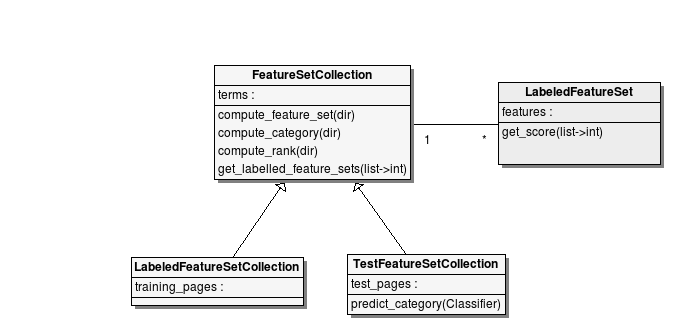
\includegraphics[scale=0.5]{figs/uml.png}
\caption{A UML class diagram describing operation of the Parser.}
\label{uml}
\end{figure}

The rest of this section talks about the specifics of the implementation, in
particular, the features used and how html parsing is done.

\paragraph{Rank mode.}
Conceptually a FeatureSetCollection is a dictionary of LabeledFeatureSet
objects indexed by both path to page and  query term. After initialisation, all
the features are computed and `filled up' per query term per page.

\paragraph{Score mode.}
\paragraph{Features.}


The requirements analysis does not prescribe the use of any particular
features. However, it states that both dynamic (query dependent) and
static(query independent) features must be used. PageRank is a dynamic feature
that has quite special place among others: it takes into account all the pages
in the pool and reflects on the structural hierarchy of the web pages. 
The parser loads the pre-computed PageRank vector indexed by page name to
extract the pagerank of any particular page.

An example of a dynamic feature used in the project is query term count: the
number of times the query term occurs on the page. This is obtained directly
from the html files using the BeautifulSoup library, just like for the link
parsing in the crawler. The html is parsed into clean text and the count is
computed on the string.
A related but different feature -- stem count -- is the number of times the
stem of the word occurs in the text. This is obtained using the PorterStemmer
module in Natural Language Tool Kit (nltk) library.

Boolean features are a slightly different variety of feature, so was worth
putting in. An example of this is a presence of an image on the page.

The features have been added incrementally as the project progressed. All other
features are similar to the ones described above and are obtained using the
same methods.\todo{enumerate features here}


\section{Optimization}

One characteristic peripheral requirement for the system implemented in this
project is speed.  Even though it is not our direct goal to produce efficient
implementations, optimization could not be overlooked, because significant amount of
time is spent processing large quantities of data: indexing, pagerank
and feature set computations all must complete in `feasible' time, i.e. in the
final implementation the longest computation takes order of minutes and
processes a few thousand pages. Various optimizations have been used to achieve
this.

Both pagerank vector and the index are precomputed and kept in persistent
storage. Incremental indexing feature allows us to edit parts of the index as
opposed to recomputing the whole index from scratch. These precomputations
provide certain speedups, but were not enough.

Because the system is fairly complex and a lot of library code is used in
places, it was hard to determine which code most affects the speed. `Blind'
attempts at optimization did not work well, which motivated the use of a
profiling tool.

Profiling the first prototype of the complete system revealed a surprising
fact: most time was spent in the library code parsing pages. To mitigate this
issue I have tried using custom parsers instead. Apart from speed, robustness
was another important consideration, as a failure of a parser increases compute
time. Two of the most renowned python parsers are html5lib and lxml. 
Figure \ref{parsers} below shows visual representation of time profiling
of 3 different runs obtained using the RunSnakeRun, each exploiting a
different parser. 
Despite html5lib being quoted as the most robust/lenient, lxml was sufficiently
faster to be preferable.

\begin{figure}
\centering
\begin{subfigure}[b]{.3\textwidth}
  \centering
  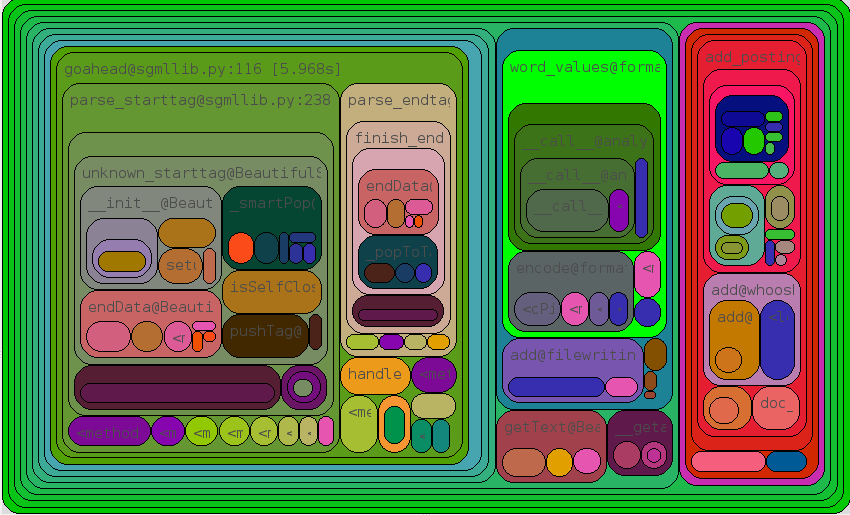
\includegraphics[width=\linewidth]{figs/prof.png}
  \caption{Default}
  \label{def}
\end{subfigure}
\quad
\begin{subfigure}[b]{.3\textwidth}
  \centering
  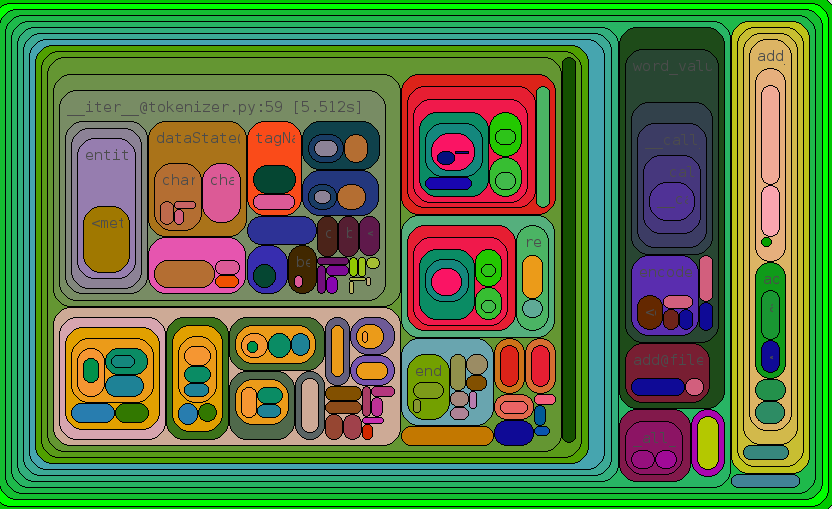
\includegraphics[width=\linewidth]{figs/html5.png}
  \caption{html5lib}
  \label{html}
\end{subfigure}
\quad
\begin{subfigure}[b]{.3\textwidth}
  \centering
  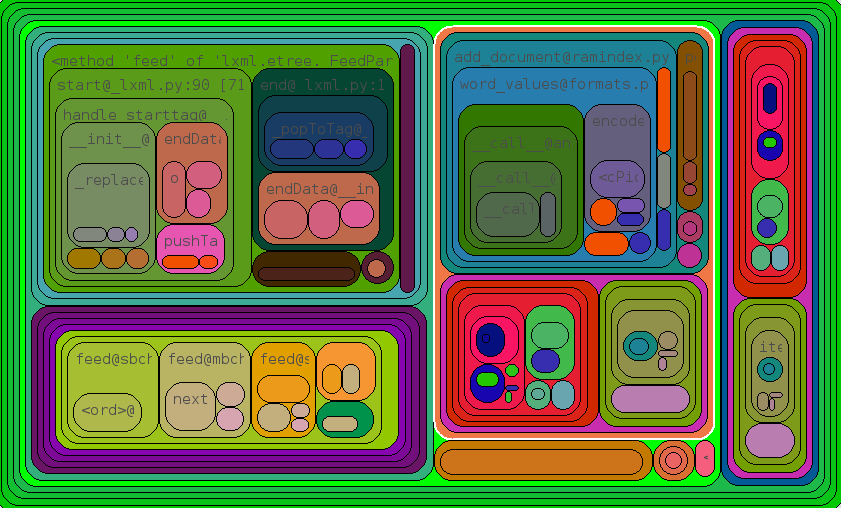
\includegraphics[width=\linewidth]{figs/lxml.png}
  \caption{lxml}
  \label{lxml}
\end{subfigure}
\caption{Visual profiles of three parsers from left to right: default python
html parser, html5lib and lxml. The internal boxes are sized in proportion to
the time spent in each function. In all profiles three distinct major
compartments can be seen, the leftmost being the compartment of interest: 
time spent in parsing. Taking into consideration that the other modules are unaffected by changing the parser
implementation, it can be observed that lxml (rightmost) is the fastest and
html5lib is the slowest.\label{parsers}}
\end{figure}

Another useful limitation was discovered due to profiling. The pagerank vector
was loaded into memory every time a page was parsed: once for each page. This
clearly is undesirable. I used caching to ensure that each of the two possible
pagerank vectors (corresponding to the test and train directories) is loaded
from memory exactly once. This is achieved via a double singleton class, which
loads the vectors lazily.
\cleardoublepage
\chapter{Evaluation}

\cleardoublepage
\chapter{Conclusion}
\cleardoublepage

%%%%%%%%%%%%%%%%%%%%%%%%%%%%%%%%%%%%%%%%%%%%%%%%%%%%%%%%%%%%%%%%%%%%%
% the bibliography

\addcontentsline{toc}{chapter}{Bibliography}
\bibliography{refs}
\cleardoublepage

%%%%%%%%%%%%%%%%%%%%%%%%%%%%%%%%%%%%%%%%%%%%%%%%%%%%%%%%%%%%%%%%%%%%%
% the appendices
\appendix

\chapter{Project Proposal}

%

\title{Machine learning inference of search engine heuristics}
\subtitle{Part II Computer Science Project Proposal}
\author{K. Palyutina, St. Catharine's College \\
        Originator: Dr. Jon Crowcroft}


% Main document

\section*{\bf Introduction, The Problem To Be Addressed}
PageRank (an algorithm which is used by Google to evaluate the `importance' of a web page) is one of the most crucial factors which determine page performance in search returns. However, there are many more of such factors that are believed to become increasingly influential. Because Google's algorithm is frequently revised, changing page ranks cause web site owners to speculate about how their web pages `deserved' an upgrade or a downgrade. Despite a large interest in this area, little research has been done to determine to what degree such factors affect the performance of a page. Certain tools\footnote{For example, Woorank or SEO are the most popular Chrome extensions to assess certain page qualities.} exist which attempt to advise web masters how to `improve' their pages. However, heuristics used by such tools are not known and are possibly incomplete and no attempt has come close to accurately predicting Google rankings.

A problem of approximating algorithms which may be used by modern search engines is characterised by vast search space, which makes exhaustive search impossible and introduces the need for generalisation. Such a problem can be reduced to a classification problem, which is traditionally solved with the help of machine learning techniques. Even though machine learning finds natural application in this area, it is easy to see how it would be very hard to create a learner and apply it to, for example, Google's search engine. Naturally, one would need to have exhaustive resources to conduct such a study. Besides, machine learning has major drawbacks that would hinder such an ambitious experiment.

Firstly, there are little theoretical guarantees in this approach. Bounds, if any, referring to how much data needs to be processed to produce a `correct' classifier are very imprecise and a classifier that performs well in practice may not be `true'\footnote{A classifier is `true' if it classifies data correctly for all inputs.}. This means that if a machine learner was to be trained by the `real world' data (Google search returns), little could be said about the performance of the obtained algorithm or, indeed, the `truthfulness' of it. Not only would it give little insight into how successful the learning is, but also no guidance for improvement. 

Another similar issue is referred to as `overfitting': this describes a situation in which a classifier performs outstandingly on a particular set of data (often similar to training data), but given different data will perform as badly as random selection. This occurs when false connections between features and outputs have been made by the learner. Unfortunately, there is no single technique that will always avoid over/under-fitting\cite{domingos}.

Clearly, such limitations are hard to combat. Besides, machine learning techniques vary greatly, so clear and detailed feedback is essential to draw conclusions about the performance of a learner. Knowing how a particular technique copes with certain heuristics would be valuable, as it would allow to approach the original problem (approximating search engine heuristics reliably) in an informed way.  

In this light, this project aspires to explore how machine learning techniques can be used to infer algorithms from search engines. To battle the constraints described above I will write my own simple search engine which will be used to observe the effectiveness of different machine learning techniques (see Figure \ref{diag1}). The existence of such a search engine is vital to the project, as it offers ultimate control over the learning process. The heuristics used in the search engine will be transparent, which, for example, eliminates the dependency on continuously changing heuristics used by Google. Another advantage of this approach is the fact that only a minimal fraction of the web needs to be used. Such a `mini-internet' will reside offline, which will speed up the indexing and also allow local modification of web pages. 

\begin{figure}
\centering
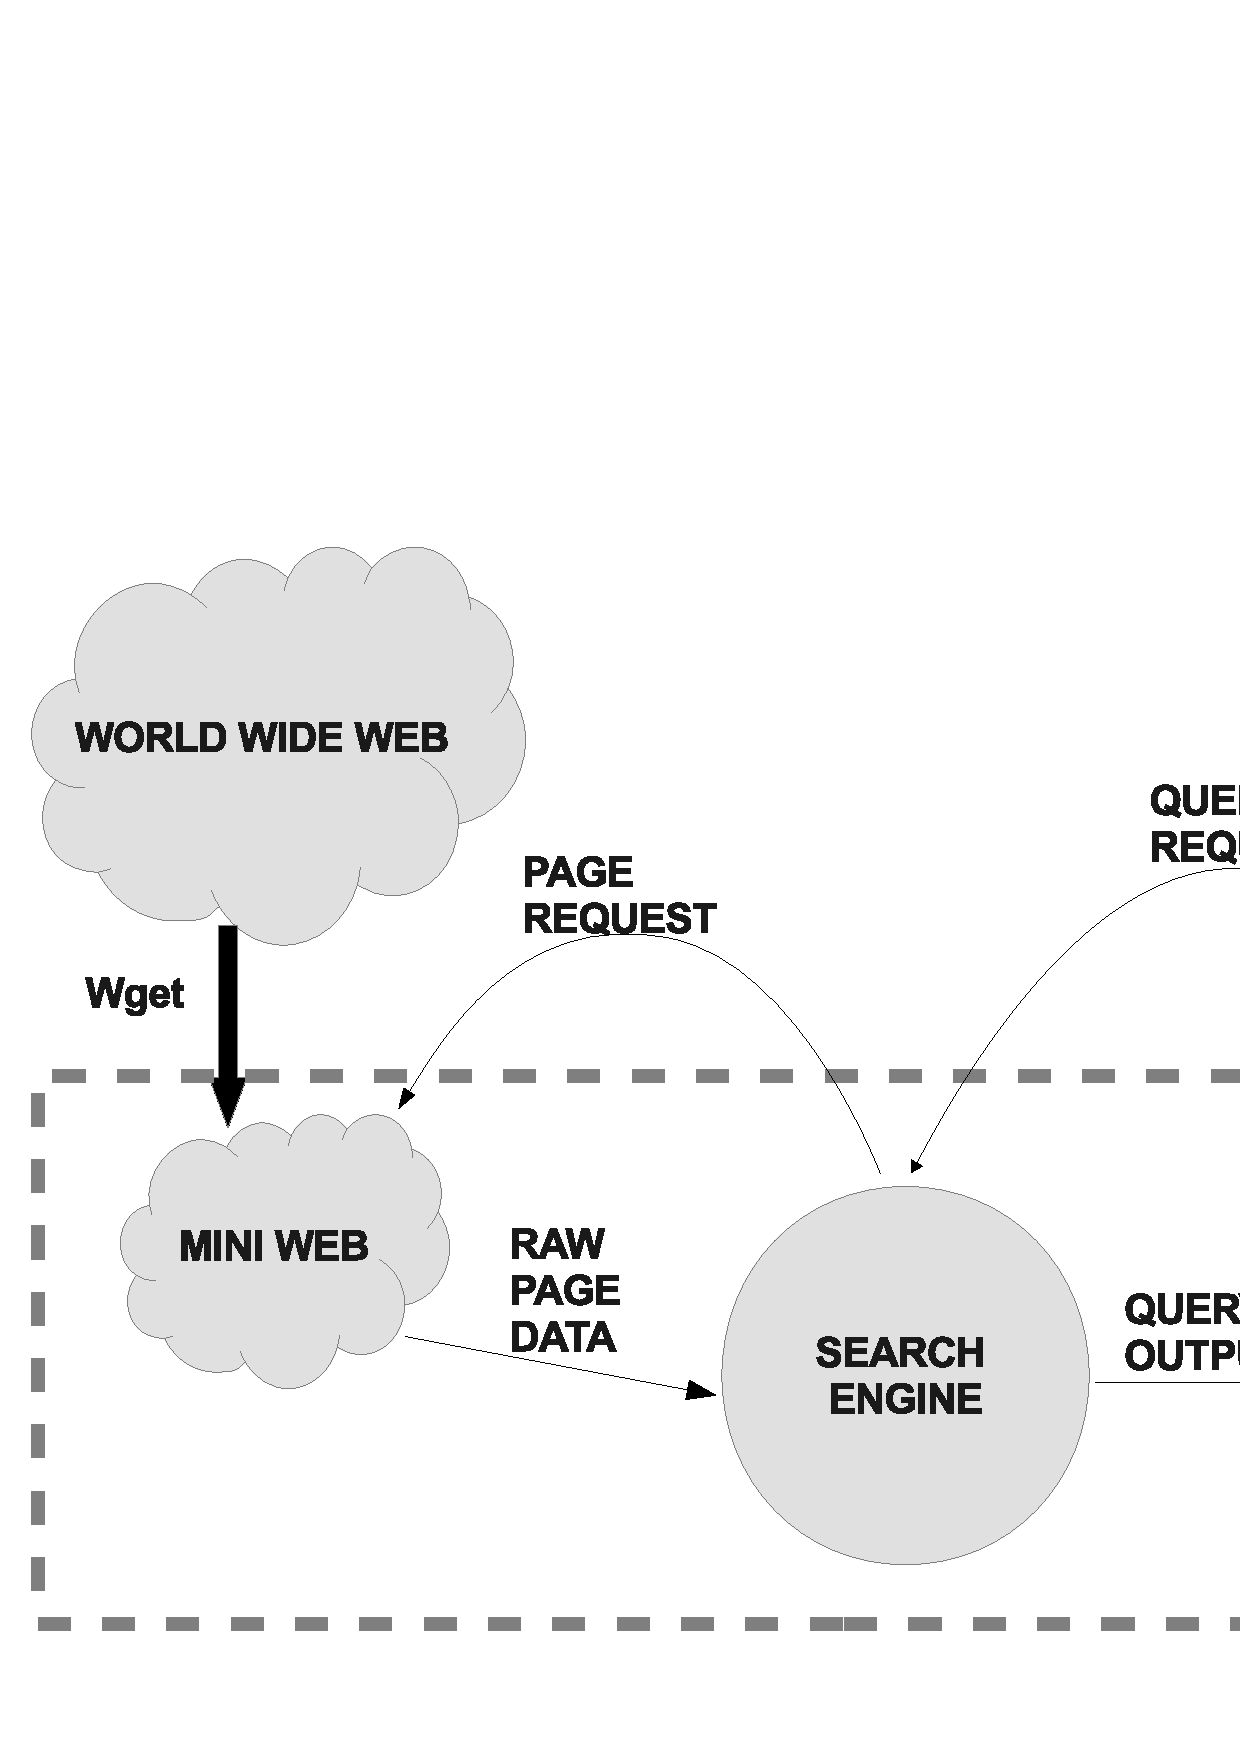
\includegraphics[scale=0.5]{diagram1}
\caption{The training of the learner. The system enclosed within the dotted box will be implemented in this project. The mini web is created by cloning web pages from the internet. The learner queries the search engine and gets back the results of the query as an input. }
\label{diag1}
\end{figure}

Most importantly, this approach gives me straightforward ways to reason about the performance of learning techniques. The search engine can be evolved to incorporate various heuristics together with PageRank. Such heuristics need not match Google's actual heuristics, however must aim to improve browsing experience \footnote{`Precision and Recall' method can be used as a guide to evaluation of search engine complexity.}. A lot of speculation has been done by web masters as to which qualities of a web page affect its ranking, these include compliance with web standards, number of words per page, frequency of occurrence of the search term on the page and alike. Because the goal of the project does not include `reverse engineering' any particular existing algorithm, there is no harm in using such guesses as guidance. 

Evolving the search engine and, hence, the learner iteratively will result in comprehensive conclusions about the effectiveness of the machine learning technique in question. Such conclusions can be used in the future as a guidance to learner design. 

\section*{\bf Starting Point}

\begin{itemize}
\item A project\footnote{\url{http://www.scienceforsearch.com/project1.asp}} was undertaken by the proposer, which developed a primitive algorithm to predict, given six characteristics of a web page, its Google ranking.  This project is mainly an inspiration, however, the speculations about the Google page ranking factors can be useful for the search engine design. 
\item Python packages exist for manipulating web pages.
\item Wget is a Linux open source utility that can be used to clone web pages.
\item The paper describing PageRank is published and will be used to implement the algorithm.
\end{itemize}


\section*{\bf Resources Required}
\begin{itemize}
\item For this project I shall mainly use my own dual-core computer that runs Ubuntu Linux. I accept full responsibility for this machine and I have made contingency plans to protect myself against hardware and/or software failure.
\item Backup will be to a BitBucket repository and/or an external hard drive.
\item I will work on MCS computers should my main machine suddenly fail. 
\end{itemize}
\section*{\bf Work to be done}

The project breaks down into the following sub-projects:

\begin{enumerate}
\item Decide on a category of search terms to explore in order to create a small network consisting of relevant web pages.

\item Implement PageRank within this network. 

\item Write a simple search engine incorporating PageRank and few other features. 

\item Decide on the representation of the input for the learner and set up the framework to format it. 

\item In advance set aside training and test data: this is necessary to then justify the evaluation of the classifier.

\item Write a simple prototype for the learner\footnote {A Naive Bayesian would be a good prototype to use.} to test the grounds. Evaluate its performance to then set goals for the final learner.  

\item Design, implement and test the learner. 

\item Attempt to evolve the search engine to be more usable and complex and observe how the learner copes with the changes of the search engine. 


\end{enumerate}

\section*{\bf Success Criterion for the Main Result}


The project will be a success if... 
\begin{itemize}
\item The resulting classifier can identify the importance of the PageRank factor in the given search engine.
\item The results of the experiment show how the chosen machine learning technique deals with various search engine heuristics. I would especially like to observe that certain heuristics are harder to pick up on than others and vice versa.
\end{itemize}
\section*{\bf Possible Extensions}
If I achieve my main result early I shall experiment with other machine learning techniques to see which perform better. I could also apply my learner to real search engines such as Google and Bing in the hope of 
discovering dependencies between features of the page and its success in ranking results.
\section*{\bf Timetable: Work plan and Milestones to be achieved.}


Planned starting date is 19/10/2011.

\begin{enumerate}

\item {\bf 9 Oct - 19 Oct:} 
\begin{itemize}
\item Do preliminary reading.
\item Familiarize myself with the field of machine learning.
\end{itemize} 
{\bf Milestone: } Complete project proposal. 
\item {\bf Oct 20 - Nov 3:} 
    \begin{itemize}
    \item Decide which and how many websites should be cloned for use as the mini web.  
    \item Prepare some training data and, separately, test data. This includes queries to be run on the search engine and expected results. 
    \end{itemize}
\item {\bf Nov 4 - Nov 15:} 
    \begin{itemize}
    \item Start writing a simple search engine and evaluate it on the test data. 
    \end{itemize}
\item {\bf Nov 15 - Nov 25:} 
    \begin{itemize}
    \item Finish the search engine.
    \item Start developing an early prototype for the learner. 
    \end{itemize} 
    {\bf Milestone: } Have a prototype of a complete system.
\item {\bf Nov 25 - Dec 15:} 
\begin{itemize}
\item Evaluate the performance of the prototype learner. 
\item Design and start implementing the final learner using the results obtained from the prototype as guidance. 
\end{itemize}
\item {\bf Dec 16 - Jan 1:} Finish the implementation of the learner. 
\item {\bf Jan 2 - Jan 16:} 
     Evaluate the resulting classifier. Here is also good time to try a different design for the learner if the classifier does not perform as well as intended.
\item {\bf Jan 17 - Feb 1:} Start working on progress report.  
{Milestone: } Write progress report. 
\item {\bf Feb 2 - Feb 20} Implement extensions.

\item {\bf Feb 20 - Mar 5:} Evaluate extensions. 

\item {\bf Mar 5 - Mar 25:} Write dissertation main chapters.

\item {\bf Mar 25 - April 10}  Further evaluation and complete dissertation.
{Milestone: } Dissertation final draft is finished.

\item {\bf April 11 - April 20:} Proof reading and submission.

\end{enumerate}


 



\end{document}
